\documentclass[11pt,a4paper]{article}

% ------------------------------------------------------------------
% Packages
% ------------------------------------------------------------------
\usepackage[utf8]{inputenc}
\usepackage[T1]{fontenc}
\usepackage{lmodern}
\usepackage[margin=2.5cm]{geometry}
\usepackage{amsmath,amssymb,mathtools}
\usepackage{booktabs}
\usepackage{graphicx}
\usepackage{xcolor}
\usepackage{listings}
\usepackage{caption}
\usepackage{algorithm}
\usepackage{algpseudocode}
\usepackage{pgfplots}
\usepgfplotslibrary{groupplots}
\pgfplotsset{compat=1.17}
\usepackage[colorlinks=true,linkcolor=blue!60!black,citecolor=blue!60!black,urlcolor=blue!60!black]{hyperref}

% ------------------------------------------------------------------
% Macros
% ------------------------------------------------------------------
\newcommand{\E}{\mathbb{E}}
\newcommand{\Q}{\mathbb{Q}}
\newcommand{\dd}{\mathrm{d}}
\newcommand{\code}[1]{\texttt{#1}}
\newcommand{\sloc}{\sigma_{\mathrm{loc}}}

% Images extracted from Model/lsv_test.ipynb by make_figures.py ; a framed placeholder is printed while a file is missing.
\newcommand{\figfile}[2]{%
  \IfFileExists{figures/#1}{\includegraphics[width=#2]{figures/#1}}%
  {\fbox{\parbox[c][4cm][c]{#2}{\centering\small missing figure:\\ \texttt{figures/#1}}}}}

\lstset{basicstyle=\ttfamily\footnotesize, keywordstyle=\color{blue!70!black}, commentstyle=\color{gray},
        stringstyle=\color{teal}, frame=single, breaklines=true, language=Python, showstringspaces=false}

\definecolor{lv}{RGB}{31,119,180}
\definecolor{mid}{RGB}{44,160,44}
\definecolor{full}{RGB}{214,39,40}
\definecolor{heston}{RGB}{90,90,90}

% ------------------------------------------------------------------
\title{A Local Stochastic Volatility Model for the CAC40:\\
Particle Calibration and Model Risk on Barriers and Autocalls}
\author{Elias Benguedda}
\date{October 2026}

\begin{document}
\emergencystretch=3em
\maketitle

\begin{abstract}
We implement a Local Stochastic Volatility (LSV) model on the CAC40 of 12 February 2025: the spot follows a local
volatility scaled by the square root of a Heston variance, $\dd S/S = \mu\,\dd t + L(t,S)\sqrt{v_t}\,\dd W$, and the
leverage function $L$ is calibrated with the particle method of Guyon and Henry-Labordère so that the model reprices
the Dupire local volatility of an SSVI fit of the market surface. A mixing fraction $\eta \in [0,1]$ scales the
volatility of variance: $\eta = 0$ is the pure local volatility model, $\eta = 1$ keeps the vol-of-vol of the
calibrated Heston model. The calibration takes 13 seconds with 50{,}000 particles on a weekly grid up to 4.86 years;
the model reprices the 142 market quotes with an implied volatility RMSE of 0.25 vol point (0.43 for Heston), of
which 0.09 is numerical error with respect to its SSVI target. At identical vanilla prices, the up-and-out call
(strike 8000, barrier 8800, one year) is worth 34.6 in local volatility and 64.7 in LSV with $\eta = 1$, the
down-and-out call 423.3 and 408.5, and the fair coupon of a 4-year Phoenix moves from 7.31\% to 6.26\% a year, while
the Athena coupon moves by 0.2 point only. These differences are model risk: vanillas do not identify $\eta$.
\end{abstract}

\tableofcontents
\newpage

% ==================================================================
\section{Introduction}
% ==================================================================
Two families of models dominate equity derivatives pricing. \emph{Local volatility} \cite{dupire1994} reprices every
vanilla option exactly, but its dynamics are poor: the forward smile flattens and the volatility is a deterministic
function of the spot. \emph{Stochastic volatility}, such as Heston \cite{heston1993}, has realistic dynamics but
only a few parameters: on the CAC40 surface of 12 February 2025, the calibrated Heston model of
\cite{benguedda2026heston} leaves an implied volatility RMSE of 0.42 vol point, with errors up to 0.8 point on the
long maturities.

The \emph{Local Stochastic Volatility} model combines both \cite{lipton2002,ren2007}: a leverage function $L(t,S)$
multiplies a stochastic volatility $\sqrt{v_t}$ and is chosen so that the model reprices the market. It is the
market standard for path-dependent equity products such as barriers and autocalls \cite{bergomi2016}. The share of
volatility carried by the stochastic part, governed here by a mixing fraction $\eta$, is not identified by vanillas:
all values of $\eta$ give the same vanilla prices but different exotic prices.

This report documents the implementation (Section~\ref{sec:method}), checks the calibration
(Section~\ref{sec:calibration}) and measures the model risk on the barrier options and autocallable notes of the
companion reports \cite{benguedda2026barrier,benguedda2026autocall} (Section~\ref{sec:risk}).

% ==================================================================
\section{Model}\label{sec:model}
% ==================================================================

\subsection{Forward log-moneyness}
Rates and dividends are deterministic and enter through the forward curve $F(0,t)$ bootstrapped from put--call parity
\cite{benguedda2026heston}. The state variable is the forward log-moneyness $y_t = \ln(S_t / F(0,t))$:
\begin{equation}
\dd y_t = -\tfrac12 \sigma_t^2\,\dd t + \sigma_t\,\dd W^S_t, \qquad \E[S_t] = F(0,t),
\end{equation}
where $\sigma_t$ is the instantaneous volatility of the spot. Implied volatilities are functions of $(y, T)$ with
$y = \ln(K/F(0,T))$, and $w(y, T) = \sigma_{\mathrm{imp}}^2(y,T)\,T$ is the total implied variance.

\subsection{Dupire local volatility}
The local volatility model $\sigma_t = \sloc(t, y_t)$ reprices the implied surface if \cite{dupire1994,gatheral2006}
\begin{equation}\label{eq:dupire}
\sloc^2(T, y) = \frac{\partial_T w}{1 - \frac{y}{w}\partial_y w + \frac14\left(-\frac14 - \frac1w + \frac{y^2}{w^2}\right)(\partial_y w)^2 + \frac12 \partial_{yy} w}.
\end{equation}

\subsection{Local stochastic volatility}
\begin{equation}
\sigma_t = L(t, y_t)\sqrt{v_t}, \qquad \dd v_t = \kappa(\theta - v_t)\,\dd t + \eta\,\xi\sqrt{v_t}\,\dd W^v_t, \qquad
\dd\langle W^S, W^v\rangle_t = \rho\,\dd t,
\end{equation}
with $(v_0, \theta, \kappa, \xi, \rho)$ the parameters of the calibrated Heston model (Table~\ref{tab:heston}) and
$\eta \in [0,1]$ the mixing fraction. By Gyöngy's theorem \cite{gyongy1986}, the one-dimensional marginals of $y_t$
are those of the local volatility model, hence the vanilla prices are the same, if and only if
\begin{equation}\label{eq:gyongy}
L^2(t, y)\; \E[v_t \mid y_t = y] = \sloc^2(t, y).
\end{equation}
For $\eta = 0$ the variance is deterministic, $\E[v_t \mid y_t] = v_t$, and the model is the local volatility model.
For $\eta = 1$ and $L \equiv 1$ it is the Heston model.

\begin{table}[h]
\centering
\begin{tabular}{@{}cccccc@{}}
\toprule
$v_0$ & $\theta$ & $\kappa$ & $\xi$ & $\rho$ & Heston IV RMSE \\
\midrule
0.0197 & 0.0438 & 1.308 & 0.482 & $-0.605$ & 0.421 vol pts \\
\bottomrule
\end{tabular}
\caption{Stochastic variance parameters: the Heston model calibrated on the CAC40 surface \cite{benguedda2026heston}.}
\label{tab:heston}
\end{table}

% ==================================================================
\section{Numerical Method}\label{sec:method}
% ==================================================================

\subsection{Smooth implied surface}
Equation~\eqref{eq:dupire} needs a surface smooth in $y$ and $T$ and free of arbitrage. The 142 quotes (13 expiries
from 9 days to 4.86 years) are fitted by:
\begin{itemize}
\item \textbf{SSVI} \cite{gatheral2014}: $w(y, T) = \frac{\theta_T}{2}\big(1 + \rho_s \varphi y + \sqrt{(\varphi y + \rho_s)^2 + 1 - \rho_s^2}\big)$,
$\varphi = \eta_s / (\theta_T^{\gamma}(1+\theta_T)^{1-\gamma})$, with the market ATM total variance $\theta_T$
(non-decreasing) and three global parameters $\rho_s = -0.454$, $\eta_s = 1.376$, $\gamma = 0.418$, chosen in the
region free of butterfly arbitrage; RMSE 0.218 vol point;
\item \textbf{SVI}: one 5-parameter smile per expiry, total variance linear in $T$ at fixed $y$ between expiries;
RMSE between 0.003 and 0.079 vol point per expiry.
\end{itemize}
SSVI is the default: its fit is coarser, but its slices never cross and its local volatility is regular in maturity,
whereas the SVI slices of the long maturities are unstable.

\subsection{Local volatility}
The derivatives of~\eqref{eq:dupire} are central finite differences of the fitted surface ($\Delta y = 10^{-3}$,
$\Delta T = 10^{-4}$). The denominator is floored at $10^{-3}$ and the local volatility clipped to $[3\%, 150\%]$
to stay finite in the far wings.

\subsection{Particle calibration of the leverage}
The conditional expectation of~\eqref{eq:gyongy} is unknown: it is estimated on the simulation itself
(Algorithm~\ref{alg:particles}, \cite{guyon2012}).

\begin{algorithm}[h]
\caption{Particle calibration of the leverage function}
\label{alg:particles}
\begin{algorithmic}[1]
\State $N$ particles $y^{(n)} = 0$, $v^{(n)} = v_0$; time grid $t_i = i\,\Delta t$, $\Delta t = 1/52$, up to $T_{\max} = 4.86$
\For{$i = 0, \dots, M$}
  \State grid $\{g_j\}_{j=1}^{60}$ between the 0.05\% and 99.95\% quantiles of the $y^{(n)}$
  \State $h = 1.5\,\mathrm{std}(y)\,N^{-1/5}$, \quad $m_j = \dfrac{\sum_n K_h(y^{(n)} - g_j)\, v^{(n)+}}{\sum_n K_h(y^{(n)} - g_j)}$ \Comment{Gaussian kernel}
  \State $L(t_i, g_j) = \sloc(t_i, g_j) / \sqrt{m_j}$
  \State move every particle by one Euler step with $\sigma^{(n)} = L(t_i, y^{(n)})\sqrt{v^{(n)+}}$ (linear interpolation in $y$)
\EndFor
\end{algorithmic}
\end{algorithm}

At $t = 0$ all particles sit at $y = 0$ and $\E[v_0 \mid y] = v_0$. For $\eta = 0$ the regression is not needed. The
variance follows an Euler full truncation scheme. The leverage is stored on the calibration grid and read at the
last calibration date before $t$ by the pricing simulation, which uses independent paths (no reuse of the particles,
hence no in-sample bias).

\subsection{Pricing}
\code{LSVModel.generate\_paths} returns the spot and its instantaneous variance $L^2 v$, the interface of the Heston
model: the Monte Carlo pricer, the Greeks and every product of the companion reports apply unchanged. The continuous
barriers use the Brownian bridge with the variance $L^2 v$ of each step \cite{benguedda2026barrier}.

\subsection{Cost}
The calibration costs $\mathcal{O}(M N G)$ in time for the kernel regressions ($M = 253$ steps, $N$ particles,
$G = 60$ grid points) and $\mathcal{O}(N G)$ in memory for the kernel weights of one step, the particles not being
stored along time; the leverage itself takes $\mathcal{O}(MG)$. Measured times: 0.6 s for $\eta = 0$, 13 s for
$\eta = 1$ with $N = 50{,}000$ (Table~\ref{tab:convergence}); about 7 s to reprice the 142 quotes on 100{,}000 daily
paths up to 4.86 years. A Vega or Volga of an LSV model recalibrates the leverage twice.

% ==================================================================
\section{Calibration Results}\label{sec:calibration}
% ==================================================================

\subsection{Local volatility}
Table~\ref{tab:localvol} and Figure~\ref{fig:localvol} show the SSVI local volatility. The local skew is about twice
the implied skew, and the short-dated wings exceed 40\% at $-30\%$ of moneyness.

\begin{table}[h]
\centering
\begin{tabular}{@{}lrrrrrr@{}}
\toprule
$T$ \textbackslash{} $y$ & $-30\%$ & $-20\%$ & $-10\%$ & $0\%$ & $+10\%$ & $+20\%$ \\
\midrule
0.1 & 43.90 & 36.13 & 26.29 & 13.36 & 15.04 & 21.29 \\
0.5 & 34.74 & 28.95 & 22.02 & 14.61 & 12.76 & 16.30 \\
1   & 29.89 & 25.16 & 19.78 & 14.47 & 12.22 & 13.99 \\
2   & 28.79 & 24.68 & 20.29 & 16.21 & 13.84 & 14.08 \\
4   & 25.65 & 22.52 & 19.35 & 16.48 & 14.49 & 13.86 \\
\bottomrule
\end{tabular}
\caption{Dupire local volatility (\%) of the SSVI surface.}
\label{tab:localvol}
\end{table}

\begin{figure}[h]
\centering
\figfile{local_vol.png}{\textwidth}
\caption{Left: SSVI local (solid) and implied (dashed) volatilities. Middle: SVI local volatility. Right: SSVI local
volatility surface.}
\label{fig:localvol}
\end{figure}

\subsection{Leverage function}
Figure~\ref{fig:leverage} shows the calibrated leverage. With $\eta = 1$, beyond six months it stays between 0.8 and
1.2 for $|y| \le 20\%$: the Heston model already explains most of the surface, and $L$ corrects its residual errors.
Short-dated leverage is larger in the wings, where the local volatility is steep; outside the particle quantiles it is
extrapolated flat. With $\eta = 0.5$ the stochastic part carries less of the smile and the leverage is more
convex.

\begin{figure}[h]
\centering
\figfile{leverage.png}{\textwidth}
\caption{Calibrated leverage $L(t, y)$ for $\eta = 1$ and $\eta = 0.5$, and leverage surface for $\eta = 1$.}
\label{fig:leverage}
\end{figure}

\subsection{Gyöngy condition}
On 100{,}000 independent pricing paths, the conditional expectation of the spot variance $\E[L^2 v_t \mid y_t = y]$,
estimated by kernel regression between the 2\% and 98\% quantiles of $y_t$, is compared with $\sloc^2$
(Figure~\ref{fig:gyongy}): the maximum gap on this range is 0.60, 0.58, 0.93 and 1.81 vol points at $t = 0.25$, 1, 2
and 4 years, the largest gaps being in the wings where few particles lie.

\begin{figure}[h]
\centering
\figfile{gyongy.png}{\textwidth}
\caption{Gyöngy check: $\sqrt{\E[L^2 v_t \mid y]}$ on the pricing paths (dots) and Dupire local volatility (line).}
\label{fig:gyongy}
\end{figure}

\subsection{Repricing of the market}
Table~\ref{tab:repricing} gives the implied volatility RMSE of each model on the market quotes (100{,}000 paths,
daily steps). Local volatility and LSV divide the Heston error by 1.7 over the whole surface, and by 1.8 to 3.5 on
the three longest maturities, where Heston is the least accurate. The remaining error is mostly the SSVI fit error:
the RMSE with respect to the SSVI target is 0.088 vol point (Table~\ref{tab:convergence}). The 9-day expiry is the
least accurate for the LSV models (0.26 and 0.41 vol point), since the leverage is calibrated on a weekly grid.

\begin{table}[h]
\centering
\begin{tabular}{@{}lrrrr@{}}
\toprule
\textbf{Expiry (y)} & \textbf{Heston} & \textbf{Local vol} & \textbf{LSV $\eta = 0.5$} & \textbf{LSV $\eta = 1$} \\
\midrule
0.025 & 0.681 & 0.138 & 0.263 & 0.414 \\
0.101 & 0.132 & 0.216 & 0.239 & 0.231 \\
0.178 & 0.122 & 0.214 & 0.239 & 0.179 \\
0.351 & 0.175 & 0.187 & 0.193 & 0.083 \\
0.600 & 0.161 & 0.203 & 0.216 & 0.119 \\
0.849 & 0.227 & 0.137 & 0.168 & 0.076 \\
1.099 & 0.097 & 0.217 & 0.217 & 0.187 \\
1.348 & 0.210 & 0.339 & 0.331 & 0.334 \\
1.597 & 0.206 & 0.110 & 0.129 & 0.113 \\
1.847 & 0.248 & 0.119 & 0.130 & 0.140 \\
2.844 & 0.634 & 0.225 & 0.237 & 0.232 \\
3.841 & 0.786 & 0.430 & 0.444 & 0.457 \\
4.858 & 0.799 & 0.237 & 0.221 & 0.227 \\
\midrule
All quotes & 0.428 & 0.230 & 0.246 & 0.245 \\
\bottomrule
\end{tabular}
\caption{Implied volatility RMSE on the 142 market quotes (vol points, Monte Carlo).}
\label{tab:repricing}
\end{table}

\begin{figure}[h]
\centering
\figfile{smiles.png}{\textwidth}
\caption{Market smiles (stars) and smiles of the four models at 9 days, 4 months, 1.1 years and 4.9 years.}
\label{fig:smiles}
\end{figure}

\subsection{Convergence}
Table~\ref{tab:convergence} shows the effect of the number of particles for $\eta = 1$. The time is linear in $N$;
the numerical error decreases from 0.147 to 0.083 vol point between 10{,}000 and 100{,}000 particles, and 50{,}000
particles are within 0.005 point of the 100{,}000 result.

\begin{table}[h]
\centering
\begin{tabular}{@{}rrrr@{}}
\toprule
\textbf{Particles} & \textbf{Calibration time (s)} & \textbf{RMSE vs SSVI} & \textbf{RMSE vs market} \\
\midrule
10{,}000 & 2.3 & 0.147 & 0.251 \\
25{,}000 & 6.3 & 0.108 & 0.246 \\
50{,}000 & 13.0 & 0.088 & 0.245 \\
100{,}000 & 26.5 & 0.083 & 0.242 \\
\bottomrule
\end{tabular}
\caption{Particle calibration, $\eta = 1$ (vol points).}
\label{tab:convergence}
\end{table}

% ==================================================================
\section{Model Risk}\label{sec:risk}
% ==================================================================
Six models price the same products: the Heston model and the LSV model with $\eta \in \{0, 0.25, 0.5, 0.75, 1\}$, all
calibrated to the same surface. Products: 1-year European barrier options of strike 8000 (continuous barriers, daily
steps) and the 4-year notes of \cite{benguedda2026autocall} (Athena: annual observations, snowball coupon of 8\%,
autocall at 100\%, protection at 60\%; Phoenix: quarterly, coupon barrier at 70\%, memory). 50{,}000 paths with a
common seed, without control variate (not available for the local volatility models).

\begin{table}[h]
\centering
\resizebox{\textwidth}{!}{%
\begin{tabular}{@{}lrrrrrrrr@{}}
\toprule
\textbf{Product} & \textbf{Heston} & \textbf{$\eta = 0$} & \textbf{$\eta = 0.25$} & \textbf{$\eta = 0.5$} & \textbf{$\eta = 0.75$} & \textbf{$\eta = 1$} & \textbf{LSV range} & \textbf{Std error} \\
\midrule
Put 1y ATM (vanilla) & 467.83 & 470.82 & 471.82 & 472.47 & 472.44 & 470.62 & 1.85 & 3.36 \\
Call 1y ATM (vanilla) & 491.03 & 495.69 & 496.50 & 496.73 & 496.14 & 494.28 & 2.45 & 2.53 \\
PDO, $H = 7200$ & 16.41 & 17.58 & 17.04 & 16.72 & 16.42 & 16.07 & 1.51 & 0.33 \\
PDI, $H = 7200$ & 451.42 & 453.24 & 454.78 & 455.74 & 456.02 & 454.55 & 2.78 & 3.42 \\
CDO, $H = 7200$ & 407.54 & 423.33 & 423.78 & 421.27 & 416.17 & 408.47 & 15.32 & 2.49 \\
CUO, $H = 8800$ & 63.04 & 34.58 & 37.18 & 44.28 & 54.74 & 64.73 & 30.15 & 0.67 \\
Down-and-out digital (100), $H = 7200$ & 44.44 & 42.90 & 42.92 & 43.10 & 43.60 & 44.20 & 1.30 & 0.17 \\
\midrule
Athena, European protection & 98.57 & 98.18 & 98.24 & 98.33 & 98.37 & 98.47 & 0.29 & 0.10 \\
\quad fair coupon (\% p.a.) & 9.44 & 9.72 & 9.68 & 9.61 & 9.60 & 9.52 & 0.20 & \\
Athena, American protection & 96.81 & 96.54 & 96.55 & 96.63 & 96.65 & 96.77 & 0.23 & 0.10 \\
\quad fair coupon (\% p.a.) & 11.21 & 11.27 & 11.30 & 11.26 & 11.29 & 11.20 & 0.10 & \\
Phoenix & 99.95 & 98.99 & 99.17 & 99.38 & 99.57 & 99.78 & 0.79 & 0.07 \\
\quad fair coupon (\% p.a.) & 6.06 & 7.31 & 7.06 & 6.77 & 6.53 & 6.26 & 1.05 & \\
\bottomrule
\end{tabular}}
\caption{Prices under the six models (nominal 100 for the notes). LSV range: maximum minus minimum over the five LSV
models. Std error: largest Monte Carlo standard error of the row.}
\label{tab:risk}
\end{table}

\begin{figure}[h]
\centering
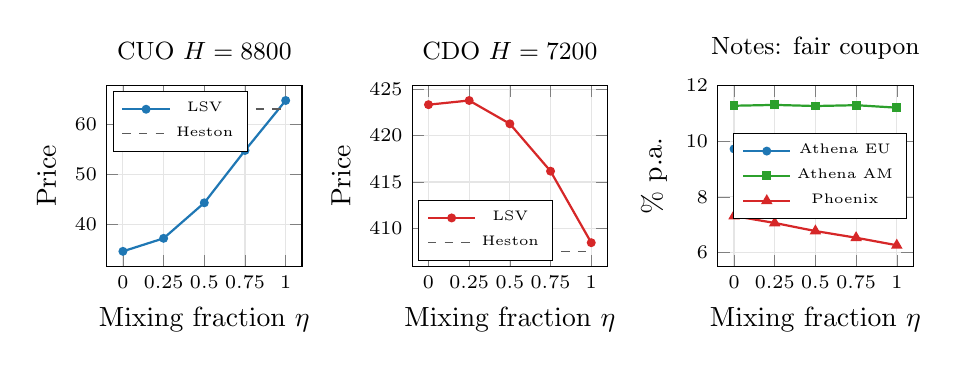
\begin{tikzpicture}
\begin{groupplot}[group style={group size=3 by 1, horizontal sep=1.4cm},
  width=0.335\textwidth, height=0.32\textwidth, xlabel={Mixing fraction $\eta$}, xtick={0,0.25,0.5,0.75,1},
  xticklabel style={font=\scriptsize}, yticklabel style={font=\scriptsize}, grid=major, grid style={gray!20},
  title style={font=\small}, legend style={font=\tiny}]
\nextgroupplot[title={CUO $H = 8800$}, ylabel={Price}, legend style={at={(0.03,0.97)}, anchor=north west}]
\addplot[lv, thick, mark=*, mark size=1.2pt] coordinates {(0,34.58) (0.25,37.18) (0.5,44.28) (0.75,54.74) (1,64.73)};
\addplot[heston, dashed] coordinates {(0,63.04) (1,63.04)};
\legend{LSV, Heston}
\nextgroupplot[title={CDO $H = 7200$}, ylabel={Price}, legend style={at={(0.03,0.03)}, anchor=south west}]
\addplot[full, thick, mark=*, mark size=1.2pt] coordinates {(0,423.33) (0.25,423.78) (0.5,421.27) (0.75,416.17) (1,408.47)};
\addplot[heston, dashed] coordinates {(0,407.54) (1,407.54)};
\legend{LSV, Heston}
\nextgroupplot[title={Notes: fair coupon}, ylabel={\% p.a.}, ymin=5.5, ymax=12, legend style={at={(0.97,0.5)}, anchor=east}]
\addplot[lv, thick, mark=*, mark size=1.2pt] coordinates {(0,9.72) (0.25,9.68) (0.5,9.61) (0.75,9.60) (1,9.52)};
\addplot[mid, thick, mark=square*, mark size=1.2pt] coordinates {(0,11.27) (0.25,11.30) (0.5,11.26) (0.75,11.29) (1,11.20)};
\addplot[full, thick, mark=triangle*, mark size=1.6pt] coordinates {(0,7.31) (0.25,7.06) (0.5,6.77) (0.75,6.53) (1,6.26)};
\legend{Athena EU, Athena AM, Phoenix}
\end{groupplot}
\end{tikzpicture}
\caption{Exotic prices as functions of the mixing fraction, at identical vanilla prices (dashed: Heston).}
\label{fig:risk}
\end{figure}

\paragraph{Vanillas.} The vanilla prices of the five LSV models differ by at most 1.85 (put) and 2.45 (call), below
the Monte Carlo standard errors (3.36 and 2.53): the mixing fraction does not change them. They are 3 to 6 above the
Heston prices, which carry the 0.42 vol point calibration error of Heston.

\paragraph{Barriers.} The up-and-out call almost doubles from $\eta = 0$ to $\eta = 1$ (34.6 to 64.7, 45 standard
errors), and the down-and-out call loses 14.9 (6 standard errors). The value of the up-and-out call comes from paths
that end between the strike and the barrier without touching it; a stochastic volatility makes low-variance scenarios
more likely, which raises this probability. Figure~\ref{fig:cuo} shows that the gap holds for every barrier level,
reaching 44.6 at $H = 9150$ between local volatility and LSV $\eta = 1$. The down-and-out put and the down-and-out digital move by 1.5 and 1.3 (5 and 8 standard
errors): far barriers on the downside depend less on the dynamics.

\paragraph{Autocalls.} The Athena is almost insensitive to $\eta$ (fair coupon 9.72\% to 9.52\%, 0.10 point with an
American protection): it depends mainly on the terminal distributions at the observation dates, which every LSV model
shares, and on the probability of a call at the first date. The Phoenix, whose coupons depend on the path above the
coupon barrier at every quarter, moves by 1.05 point of coupon (7.31\% to 6.26\%).

\paragraph{Heston.} Heston is close to LSV $\eta = 1$ on the barriers (CUO 63.0 against 64.7, CDO 407.5 against
408.5), as expected from a leverage close to 1, but its notes inherit its vanilla errors (Phoenix fair coupon 6.06\%
against 6.26\%).

\begin{figure}[h]
\centering
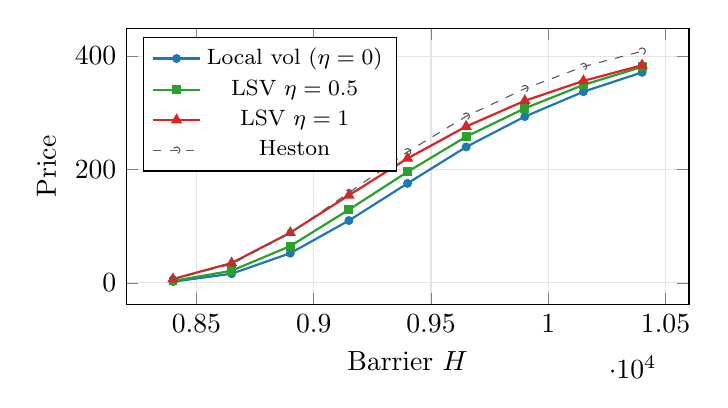
\begin{tikzpicture}
\begin{axis}[width=0.72\textwidth, height=0.42\textwidth, xlabel={Barrier $H$}, ylabel={Price},
             grid=major, grid style={gray!20}, legend pos=north west, legend style={font=\footnotesize},
             xticklabel style={/pgf/number format/1000 sep={}}]
\addplot[lv, thick, mark=*, mark size=1.2pt] coordinates {(8400,2.06) (8650,16.03) (8900,52.19) (9150,109.84) (9400,175.44) (9650,239.67) (9900,293.27) (10150,337.11) (10400,371.28)};
\addplot[mid, thick, mark=square*, mark size=1.2pt] coordinates {(8400,3.23) (8650,21.33) (8900,64.76) (9150,129.01) (9400,195.79) (9650,257.84) (9900,307.76) (10150,349.15) (10400,380.86)};
\addplot[full, thick, mark=triangle*, mark size=1.6pt] coordinates {(8400,6.69) (8650,34.90) (8900,88.45) (9150,154.47) (9400,219.48) (9650,275.84) (9900,321.16) (10150,356.22) (10400,383.78)};
\addplot[heston, dashed, mark=o, mark size=1.2pt] coordinates {(8400,6.32) (8650,33.08) (8900,87.76) (9150,158.98) (9400,231.04) (9650,293.70) (9900,342.48) (10150,381.37) (10400,408.48)};
\legend{Local vol ($\eta = 0$), LSV $\eta = 0.5$, LSV $\eta = 1$, Heston}
\end{axis}
\end{tikzpicture}
\caption{Up-and-out call ($K = 8000$, $T = 1$) as a function of the barrier.}
\label{fig:cuo}
\end{figure}

% ==================================================================
\section{Greeks}\label{sec:greeks}
% ==================================================================
Table~\ref{tab:greeks} compares the Greeks of the up-and-out call and of the Athena (common random numbers, 50{,}000
paths). For the LSV models, Vega and Volga shift the whole implied surface by one vol point and recalibrate the
leverage, the market definition of a Vega; for Heston they shift $\sqrt{v_0}$ and $\sqrt{\theta}$, so the two are not
directly comparable. Delta keeps the surface fixed in moneyness.

\begin{table}[h]
\centering
\resizebox{\textwidth}{!}{%
\begin{tabular}{@{}lrrrr@{\qquad}rrrr@{}}
\toprule
 & \multicolumn{4}{c}{\textbf{CUO 1y, $H = 8800$}} & \multicolumn{4}{c}{\textbf{Athena 4y, European protection}} \\
\cmidrule(lr){2-5}\cmidrule(lr){6-9}
 & $\eta = 0$ & $\eta = 0.5$ & $\eta = 1$ & Heston & $\eta = 0$ & $\eta = 0.5$ & $\eta = 1$ & Heston \\
\midrule
Price & 34.58 & 44.28 & 64.73 & 63.04 & 98.18 & 98.33 & 98.47 & 98.57 \\
Delta (per point) & $-0.0457$ & $-0.0547$ & $-0.0491$ & $-0.0618$ & 0.00481 & 0.00491 & 0.00496 & 0.00505 \\
Gamma ($\times 10^{5}$) & $-5$ & $-8$ & $-23$ & $-21$ & $-1$ & $-1$ & $-1$ & 0 \\
Vega (per vol pt) & $-6.05$ & $-7.03$ & $-7.94$ & $-11.46$ & $-0.575$ & $-0.557$ & $-0.527$ & $-0.534$ \\
Volga & 1.45 & 1.71 & 1.16 & 1.79 & $-0.035$ & $-0.002$ & $-0.045$ & $-0.040$ \\
Rho (per 1\%) & $-1.24$ & $-1.53$ & $-1.97$ & $-1.45$ & $-0.743$ & $-0.803$ & $-0.748$ & $-0.774$ \\
Dividend (per 1\%) & 0.89 & 1.08 & 1.33 & 0.82 & $-1.086$ & $-1.038$ & $-1.114$ & $-1.111$ \\
Theta (per day) & 0.107 & 0.173 & 0.188 & 0.210 & 0.0086 & 0.0063 & 0.0052 & 0.0049 \\
\bottomrule
\end{tabular}}
\caption{Greeks under local volatility, LSV and Heston (168 s in total, most of it for the recalibrations of the
Vegas).}
\label{tab:greeks}
\end{table}

The Greeks of the Athena are nearly model independent (Vega $-0.53$ to $-0.58$, Dividend $-1.04$ to $-1.11$), like its
price. The up-and-out call has a negative Vega in every model, larger in absolute value when the volatility is more
stochastic, and a Gamma four times larger with $\eta = 1$ than in local volatility: hedging it with a local
volatility model would underestimate both.

% ==================================================================
\section{Implementation}\label{sec:implementation}
% ==================================================================
\begin{itemize}
\item \code{Model/local\_vol.py}: \code{LocalVolSurface} (Dupire from SSVI, SVI or a flat volatility; implied surface
shift for the Vega), \code{LSVModel} (particle calibration, \code{generate\_paths}, \code{leverage},
\code{vol\_shifted}) and \code{reprice\_surface};
\item \code{Produits/market.py}: \code{cac40\_lsv(mixing)} builds a calibrated LSV model on the CAC40;
\item \code{Model/lsv\_test.ipynb}: the notebook of this report (6 to 8 minutes).
\end{itemize}

\begin{lstlisting}
from market import cac40_heston, cac40_lsv
from products import BarrierOption, Phoenix
from monte_carlo import MonteCarloPricer

mkt = cac40_heston()
lsv = cac40_lsv(mkt, mixing=0.5)                      # Dupire (SSVI) + leverage, 50,000 particles
pricer = MonteCarloPricer(n_paths=50_000, steps_per_year=252, seed=42, control_variate=False)
print(pricer.price(lsv, BarrierOption.from_code("CUO", 8000, 8800, 1.0)))
note = Phoenix(4.0, mkt.S0, 0.06, coupon_barrier=0.7, frequency=0.25)
print(note.fair_coupon(MonteCarloPricer(n_paths=50_000, steps_per_year=52, seed=42, control_variate=False), lsv))
\end{lstlisting}

% ==================================================================
\section{Limitations and Next Steps}\label{sec:limitations}
% ==================================================================
\begin{itemize}
\item \emph{Mixing fraction.} Vanillas do not identify $\eta$; it must be calibrated to exotic quotes (barriers,
forward-start options, VIX-type products), not available here. The model risk of Table~\ref{tab:risk} is the range
of prices compatible with the vanilla surface.
\item \emph{Implied surface.} The SSVI fit error (0.22 vol point) is inherited by every model; a richer arbitrage-free
parametrisation (e.g. eSSVI) would lower it.
\item \emph{Short maturities.} The weekly calibration grid limits the accuracy of the 9-day expiry (0.41 vol point
for $\eta = 1$); a finer grid at the start would fix it.
\item \emph{Particle method.} Kernel bias in the wings (Gyöngy gaps up to 1.8 vol points at 4 years beyond the
central quantiles), Euler scheme with the Feller condition violated; a PDE calibration (Fokker--Planck) is the
standard alternative.
\item \emph{Dynamics.} Sticky-moneyness spot bumps; one stochastic factor; no stochastic rates or dividends.
\end{itemize}

% ==================================================================
\section{Conclusion}
% ==================================================================
A Local Stochastic Volatility model calibrated by the particle method reprices the CAC40 surface with an implied
volatility RMSE of 0.25 vol point, against 0.43 for Heston, in 13 seconds. At identical vanilla prices, the mixing
fraction moves the up-and-out call by a factor of two, the down-and-out call by 15 and the Phoenix fair coupon by one
point of coupon, while the Athena moves by 0.2 point: path-dependent products whose value depends on the path between
observation dates or near a barrier carry a model risk that vanilla calibration alone cannot remove.

% ==================================================================
\appendix
\section{Notation}
% ==================================================================
\begin{center}
\begin{tabular}{@{}ll@{}}
\toprule
Symbol & Meaning \\
\midrule
$y = \ln(S/F(0,t))$ & Forward log-moneyness \\
$w(y, T)$ & Total implied variance $\sigma_{\mathrm{imp}}^2 T$ \\
$\sloc(t, y)$ & Dupire local volatility \\
$L(t, y)$ & Leverage function \\
$v_t$; $(v_0, \theta, \kappa, \xi, \rho)$ & Stochastic variance and its parameters \\
$\eta$ & Mixing fraction (share of the vol-of-vol kept) \\
$N$, $M$, $G$, $h$ & Particles, time steps, regression grid points, kernel bandwidth \\
\bottomrule
\end{tabular}
\end{center}

% ==================================================================
\begin{thebibliography}{99}
\bibitem{benguedda2026heston} E. Benguedda, \emph{Calibration of the Heston Stochastic Volatility Model: Theoretical
Framework, Numerical Methods, and Limitations}, 2026.
\bibitem{benguedda2026barrier} E. Benguedda, \emph{Monte Carlo Pricing and Greeks of Single Barrier Options under a
Calibrated Heston Model}, 2026.
\bibitem{benguedda2026autocall} E. Benguedda, \emph{Autocallable Notes on the CAC40 under a Calibrated Heston Model:
Athena and Phoenix}, 2026.
\bibitem{dupire1994} B. Dupire, Pricing with a smile, \emph{Risk}, 7(1):18--20, 1994.
\bibitem{heston1993} S. L. Heston, A closed-form solution for options with stochastic volatility with applications
to bond and currency options, \emph{Review of Financial Studies}, 6(2):327--343, 1993.
\bibitem{gatheral2006} J. Gatheral, \emph{The Volatility Surface: A Practitioner's Guide}, Wiley, 2006.
\bibitem{gatheral2014} J. Gatheral and A. Jacquier, Arbitrage-free SVI volatility surfaces, \emph{Quantitative
Finance}, 14(1):59--71, 2014.
\bibitem{gyongy1986} I. Gyöngy, Mimicking the one-dimensional marginal distributions of processes having an Itô
differential, \emph{Probability Theory and Related Fields}, 71(4):501--516, 1986.
\bibitem{guyon2012} J. Guyon and P. Henry-Labordère, Being particular about calibration, \emph{Risk}, 25(1):88--93,
2012.
\bibitem{lipton2002} A. Lipton, The vol smile problem, \emph{Risk}, 15(2):61--65, 2002.
\bibitem{ren2007} Y. Ren, D. Madan and M. Q. Qian, Calibrating and pricing with embedded local volatility models,
\emph{Risk}, 20(9):138--143, 2007.
\bibitem{bergomi2016} L. Bergomi, \emph{Stochastic Volatility Modeling}, Chapman and Hall/CRC, 2016.
\end{thebibliography}

\end{document}
